\documentclass[11pt,addpoints]{exam}
\usepackage{amsfonts,amssymb,amsmath, amsthm}
\usepackage{graphicx}
\usepackage{systeme}
%\usepackage{pgf,tikz,pgfplots}
%\pgfplotsset{compat=1.15}
%\usepgfplotslibrary{fillbetween}
\usepackage{mathrsfs}
%\usetikzlibrary{arrows}
%\usetikzlibrary{calc}


\pagestyle{headandfoot}

\firstpageheader{Sample Exam (\numpoints\ points)\\ September 26, 2019}{}{Name: \underline{\hspace{2.5in}}}
%\firstpageheadrule

\runningheader{Sample Exam}{}{Page \thepage\ of \numpages}
\runningheadrule

\firstpagefooter{}{}{}
\runningfooter{}{}{}


\begin{document}

\begin{center}
\fbox{\fbox{\parbox{6in}{\centering
No notes, calculators, or other aids are allowed.  Read all directions carefully and write your answers in the space provided.  To receive full credit, you must show all of your work.
}}}
\end{center}




\begin{questions} %------------------------------------------


\fullwidth{\emph{Math mode} is used to display mathematical content in \LaTeX, and there are two main forms of math mode: \emph{display mode} and \emph{inline mode}.  Question~\ref{DisplayModeExample} uses \emph{display mode}, which centers the math content on its own line.  Question~\ref{InlineModeExample} uses \emph{inline mode} to render the math content within a line of text.}



\question[10] \label{DisplayModeExample}
Find an equation for the tangent line to the following curve at the point (0,1).
\[2xy^3 + y^4 = 1 + x^3y\]
\vspace{\stretch{1}}



\question[10] \label{InlineModeExample}
Use the linearization of $f(x) = \sqrt[3]{x}$ at $x=8$ to approximate $\sqrt[3]{8.24}$.

\vspace{\stretch{1}}





\newpage %---------------------------------------------------



\question \label{DisplaystyleExamples}
Evaluate each expression.

\begin{parts}

\part[5]
$\displaystyle\lim_{x\to\infty} \left( 1+\frac{1}{x} \right)^{x}$
\vspace{\stretch{1}}

\part[5]
$\displaystyle\frac{d}{dx} \left[ \frac{\sin^2(\pi x)}{\sqrt{3x+1}} \right]$
\vspace{\stretch{1}}

\part[5]
$\displaystyle\int_1^{e^2} t \ln t\ dt$
\vspace{\stretch{2}}

\end{parts}



\question
Using the \emph{displaystyle} command (as in each part of question~\ref{DisplaystyleExamples}) forces fractions, limits, integrals, etc. to be displayed larger and more clearly even when using inline mode.  Without \emph{displaystyle}, those math expressions will be shrunk when using inline mode, like so:

\begin{parts}

\part[5]
$\lim_{x\to\infty} \left( 1+\frac{1}{x} \right)^{x}$
\vspace{\stretch{1}}

\part[5]
$\frac{d}{dx} \left[ \frac{\sin^2(\pi x)}{\sqrt{3x+1}} \right]$
\vspace{\stretch{1}}

\part[5]
$\int_1^{e^2} t \ln t\ dt$
\vspace{\stretch{2}}

\end{parts}




\newpage %---------------------------------------------------

\question[8]
Use the Gauss-Jordan elimination method to find all solutions (if any) to the following system of equations.

\begin{equation*}
\systeme{\frac{1}{2}x + \frac{3}{2}y - 2z = 10, 2x + 2y + 4z = 24, x + 2y = 16}
\end{equation*}

\begin{align*}
\frac{1}{2}x + \frac{3}{2}y - 2z & = 10 \\
2x + 2y + 4z & = 24\\
x + 2y &= 16
\end{align*}

\vspace{\stretch{2}}



\question[4] Use the following matrices to calculate $(A+4B)C$.

\[
A = \left[\begin{matrix} 3 & 4 \\ -5 & 1 \end{matrix}\right] \qquad
B = \left[\begin{matrix} 0 & -1 \\ 1 & 0 \end{matrix}\right] \qquad
C = \left[\begin{matrix} 5 & -6 & 2 \\ 1 & 1 & -2 \end{matrix}\right].
\]
\vspace{\stretch{1}}




\newpage %---------------------------------------------------

\question[3]
The lines $2x-6y=3$ and $x+3y=9$ are $\ldots$

\begin{choices}
\choice parallel
\choice perpendicular
\choice neither A nor B
\end{choices}

\vspace{\stretch{1}}



\question[3]
Which of the following expressions are equivalent to $\ln(16)$?  Circle all that apply.

\begin{oneparchoices}
\choice $\ln(20)-\ln(4)$
\choice $\ln(\frac{1}{2})+\ln(32)$
\choice $\ln(2)\cdot\ln(8)$
\choice $2\ln(4)$
\end{oneparchoices}

\vspace{\stretch{1}}



\question[2]
If $f''(x)$ is \fillin[negative][4cm] on some interval, then the graph of $f$ is concave down on that interval.

\vspace{\stretch{1}}



\question[2]
What is the name for the set of all valid inputs of a function?
\answerline

\vspace{\stretch{1}}



\question[4]
Sketch the graph of the piecewise function $f(x) = \displaystyle\begin{cases} 5-x^2 & \text{if } x<3 \\ x-2 & \text{if } x\ge 3 \end{cases}$.

\begin{center}
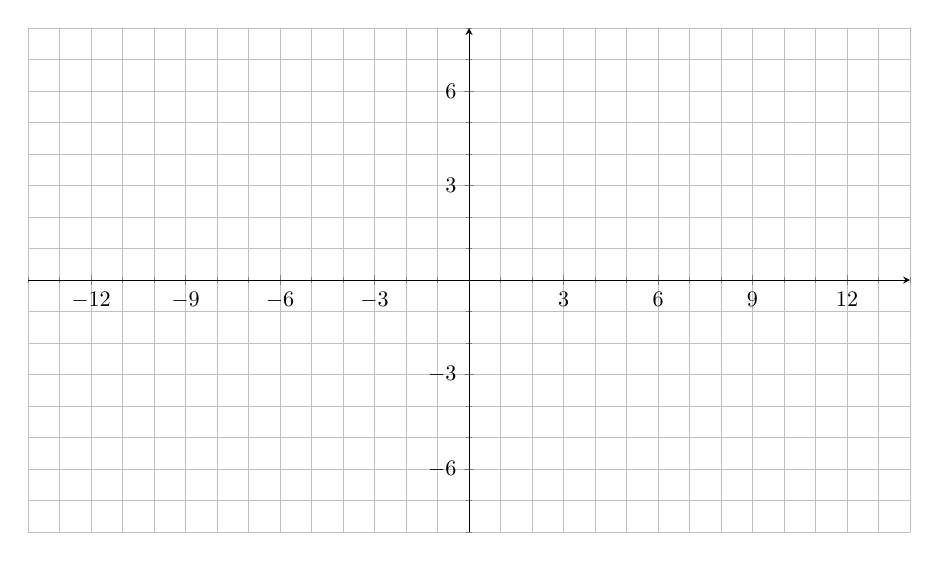
\begin{tikzpicture}[scale=0.8]

\begin{axis}[axis lines=middle,grid=both,
            xtick distance=3,ytick distance=3,minor tick num=2,
            x=0.5cm,y=0.5cm,xmin=-14,xmax=14,ymin=-8,ymax=8]
% no plots to draw ... just empty grid with axes
\end{axis}

\end{tikzpicture}
\end{center}






\newpage %---------------------------------------------------

\question[10]
A farmer wants to build two adjacent animal pens using 5 straight sections of fence, as shown below.  Which dimensions will produce the \textbf{largest total area} if the farmer has 60 feet of fence to use?

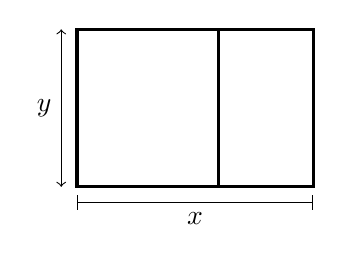
\begin{tikzpicture}

\draw[very thick] (0,0) rectangle (3,2);
\draw[very thick] (1.8,0) -- (1.8,2);

\draw[|-|,thin] (0,-0.2) -- node[below] {$x$} (3,-0.2);
\draw[<->,thin] (-0.2,0) -- node[left] {$y$} (-0.2,2);

\end{tikzpicture}

\vspace{\stretch{1}}



\question[10]
Find the area of the region enclosed by $y=x^2+2x-7$ and $y=x-1$.

\begin{flushright}
\begin{tikzpicture}[scale=0.7]

\begin{axis}[axis on top,axis lines=middle,x=0.5cm,y=0.5cm,
            xmin=-7,xmax=7,ymin=-9,ymax=5]
            
\addplot[name path=F,black,very thick,domain=-7:7,samples=100]{x^2 + 2*x - 7};
\addplot[name path=G,black,very thick,domain=-7:7]{x - 1};
\addplot[black!30] fill between[of=F and G,soft clip={domain=-3:2}];

\end{axis}

\end{tikzpicture}
\end{flushright}

\vspace{\stretch{1}}





\newpage %---------------------------------------------------

\question \LaTeX\ can display saved images in formats like JPG, PNG, PDF, and more.

\begin{center}
\includegraphics[width=4in]{unitcircle.png}
\end{center}

\begin{center}
\includegraphics[width=4in]{unitcircle.pdf}
\end{center}







\newpage %---------------------------------------------------

\question Here are a few more sample math expressions.

\[ x = \frac{-b \pm \sqrt{b^2 - 4ac}}{2a} \]

\[ \binom{n}{k} = \frac{n!}{k!(n-k)!} \]

\[ [a,b) = \{ x\in\mathbb{R} \mid a \le x < b \} \]

\[ m = \frac{\Delta y}{\Delta x} = \frac{y_2 - y_1}{x_2 - x_1} \]

\[ \int_a^b f(x)\ dx = \lim_{n\to\infty} \left( \sum_{i=1}^n f(x_i^*) \Delta x_i \right) \]

\[ \frac{d}{dx} \left[ \int_a^x f'(t)\ dt \right] = f(x) \]

\[ \sin^2\alpha + \cos^2\alpha = 1 \]

\[ e^{i\theta} = \cos\theta + i\sin\theta \]

\[ \vec{v} = \langle 2,3,-1 \rangle = 2\hat{\imath} + 3\hat{\jmath} - \hat{k} \]

\[ \overline{AB}, \overleftrightarrow{AB}, \angle ABC, \measuredangle ABC \]

\[ \triangle ABC \cong \triangle DEF \]

\[ \sim (p \lor q) \Longleftrightarrow \ \sim p \ \land \sim q \]



\end{questions}

\end{document}